\chapter{Verification and Testing}

\section{GitLab}

Make sure GitLab is accessible via https and the certificate is valid.
Just take a browser and go to 'https://gitlabtest.gruber.info' and verify the browser's response.

\begin{figure}[H]
	\centering
	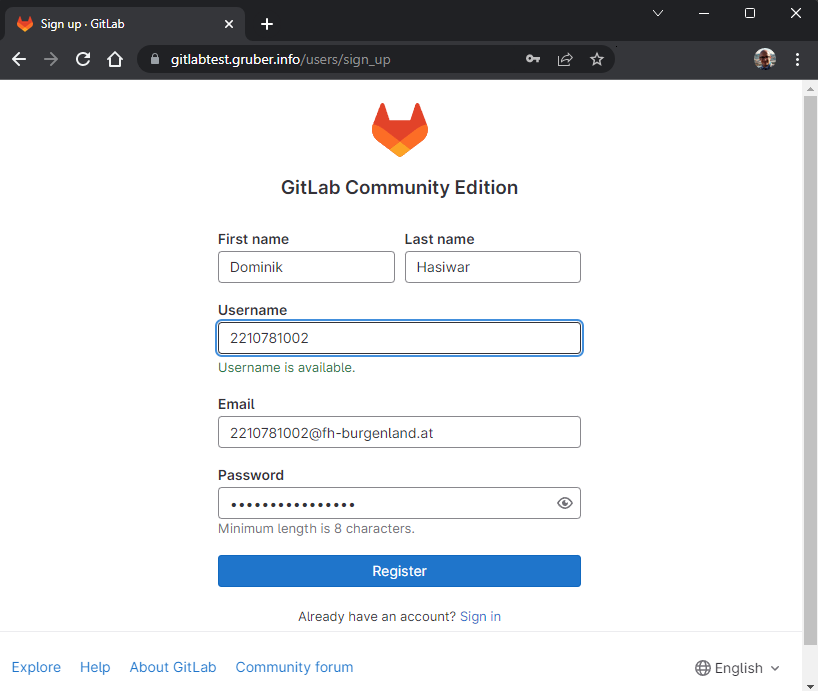
\includegraphics[width=14cm]{images/gitlab_signup.png}
	\caption{GitLab https response}
	\label{fig:gitlab_response}
\end{figure}
\  \\

The logs from GitLab can be accessed directly with the 'logs' command of 'docker compose':
\begin{lstlisting}[language=bash,caption={GitLab Logging},label={code:gitlab-logging}]
    # Open and follow to GitLab logs
    /home/debian/gitlab && docker compose logs -f
\end{lstlisting}

\section{GitLab Runners}

Verify if all added Runners are list in the Admin area of GitLab, see \ref{fig:gitlab_list_runners}.
If a Runner is not listed there, follow the 'Troubleshooting GitLab Runner' FAQ from GitLab (\cite{refGitLabRunnersTroubleshooting}).

\section{End-to-End test}

To verify all functionality all together, create a new project within GitLab, for example use the '.Net Core' template.
\begin{figure}[H]
	\centering
	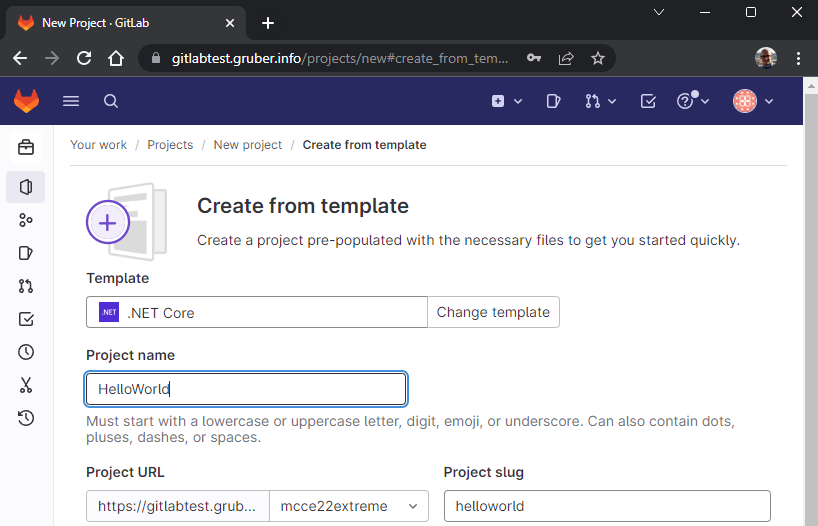
\includegraphics[width=14cm]{images/gitlab_create_project.png}
	\caption{GitLab create project}
	\label{fig:gitlab_create_project}
\end{figure}

Verify at the 'Jobs' list, if the jobs specified in the project are running successfully, see \ref{fig:gitlab_jobs_list}.
Failed jobs should be analyzed if the failure is in the infrastructure or in the code.
\begin{figure}[H]
	\centering
	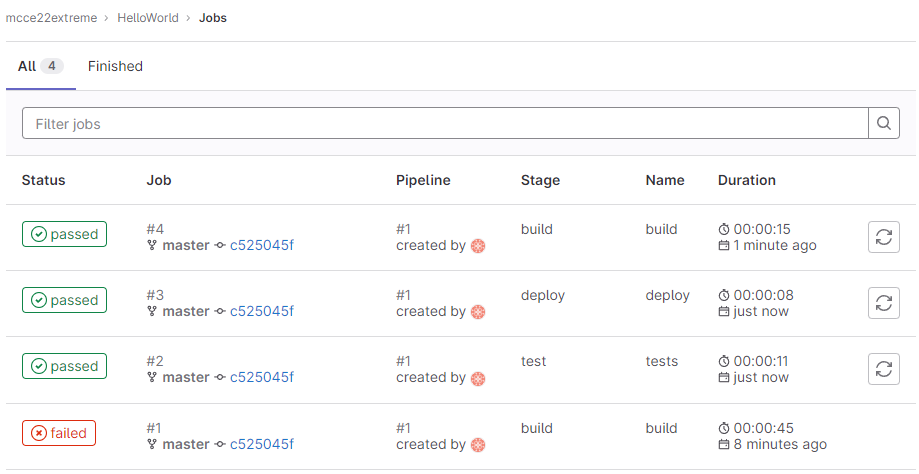
\includegraphics[width=14cm]{images/gitlab_jobs_list.png}
	\caption{List of jobs in GitLab project}
	\label{fig:gitlab_jobs_list}
\end{figure}